%!TEX root = report.tex
\exercise{Texture}
Texture measures are useful for providing statistical information about images or segments of images.

\subsection*{Measures}
The measures that we've considered are listed below.
Most of the measures use the definition of the \(n\)th moment, which is given by\cite[Eq. 11.3-4]{gonzalez2002digital}:
\[
	\mu_n(z) = 
	\sum_{i=0}^{L-1}(z_i - m)^n p(z_i)
\]
\begin{itemize}
	\item \textbf{Mean}:
	This is simply the mean intensity value of the image. It can be calculated in the conventional matter, but we've followed the method that the book suggested \cite[Eq. 11.3-5]{gonzalez2002digital}:
	\[
		m = 
		\sum_{i=0}^{L-1}z_i p(z_i)
	\]
	
	\item \textbf{Variance}:
	This is a measure of how far the values (intensities, in our case) are spread out.
	It can be calculated by taking the second moment, \(\mu_2(z)\).
	
	\item \textbf{Standard deviation}:
	The standard deviation, \(\sigma\), is actually very similar to the variance, but more intuitive for many people.
	It is simply the square root of the variance, \(\sqrt{\mu_2(z)}\).

	\item \(\mathbf{R}\):
	\(R\) is a measure of \emph{relative smoothness}.
	It is determined as follows:
	\[
	R(z) = 
	1 - \frac{1}{1 + \mu_2(z)}
	\]
	
	\item \textbf{Skewness}:
	The skewness is a measure of asymmetry in the distribution of values around the mean.
	A measure of the skewness if given by the third moment, \(\mu_3(z)\).

	\item \textbf{Flatness}:
	The flatness (or kurtosis) is a measure of how flat the peaks of the distribution of values are.
	A measure of the flatness is given by the fourth moment, \(\mu_4(z)\).

	\item \textbf{Uniformity}:
	The uniformity is a measure of how uniform the values are.
	It is given by\cite[Eq. 11.3-8]{gonzalez2002digital}:
	\[
		U(z) = \sum_{i=0}^{L-1}p^2(z_i)
	\]

	\item \textbf{Average entropy}:
	The average entropy is a measure of how much information is contained in the values, from an information theoretical point of view.
	It is given by\cite[Eq. 11.3-9]{gonzalez2002digital}:
	\[
		e(z) = -\sum_{i=0}^{L-1}p(z_i)\log_2 p(z_i)
	\]
\end{itemize}

Some of the measures have been normalized so that they give values between 0 and 1.

\subsection*{Implementation}
For the implementation, we've used the fact that all of the sums in the definitions can easily be calculated by taking the dot product of different vectors. The \(n\)th moment is implemented in the function \texttt{mu}, and the measures are calculated in the function \texttt{IPtexturemeasures}:
\matlabexternal{../mu.m}
\matlabexternal{../IPtexturemeasures.m}

\subsection*{Results}
When calculating these measures for the requested subimages of \texttt{bubbles.tif}, \texttt{cktboard.tif} and \texttt{cereal.tif}, the results in Table~\ref{tab:measures} are obtained.
The segments of the images that are measured are shown in Figure~\ref{fig:measured_images}.

\begin{figure}[htb]
 \centering
 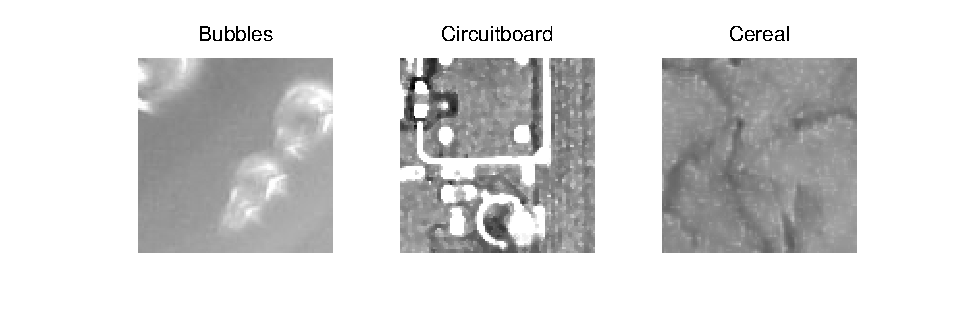
\includegraphics[width=\linewidth]{measured_images.eps}
 \caption{The measured images.}
 \label{fig:measured_images}
\end{figure}

\begin{table}[htb]
    \begin{tabular}{| r | r | r | r | r | r | r | r | r |}
	    \hline
	    \textbf{Image}    & \textbf{Mean} & \textbf{Variance} & \(\pmb{\sigma}\) & \(\mathbf{R}\) & \textbf{Skewness} & \textbf{Flatness}     & \(\mathbf{U}\) & \(\mathbf{e}\) \\ \hline
	    \texttt{bubbles}  & 165           & 0.0096            & 24.97            & 0.0095         &  0.2983           &  \(17.44 \cdot 10^5\) & 0.0179         & 6.20           \\
	    \texttt{cktboard} & 158           & 0.0398            & 50.87            & 0.0383         &  1.3299           & \(198.62 \cdot 10^5\) & 0.0384         & 5.98           \\
	    \texttt{cereal}   & 140           & 0.0031            & 14.28            & 0.0031         & -0.0208           &   \(1.29 \cdot 10^5\) & 0.0208         & 5.83           \\
	    \hline
    \end{tabular}
    \caption{The texture measures. Some decimal places have been omitted so that all measures fit on one row.}
    \label{tab:measures}
\end{table}

By looking at the images and the measures, one can confirm some of the measures visually:
\begin{itemize}
	\item
	The \texttt{cktboard} image has both very low and very high intensities.
	This indicates that it might have a hight standard deviation and variance.
	The measures of the standar deviation and variance confirm this.

	\item
	Piecewise, the \texttt{cktboard} image is rather smooth.
	The relative smoothness measure \(R\) confirms this.

	\item
	It is visible with the eye that the \texttt{cereal} image has a very `peaky' behaviour.
	The low value of the flatness confirms this.

	\item
	Empirically, we have the suspicion that skewness is related to how "regular" or how "repeating" an image is. This seems to be confirmed by that circuitboard seems to be more textured than the other two images, as well as in the book in \cite[p. 828, figure 11.28(c)]{gonzalez2002digital} seems to be more textured than the other two images and its skewness is significantly higher. However, we have no formal statistics to confirm this intuition. 
\end{itemize}

\clearpage